\documentclass[myclassdoc,debug]{rjparticle}
%use the following command when typesetting your paper:
%\documentclass{rjparticle}
\usepackage{graphicx}

\title{Extensive Study of the Positive and Negative Parity Wobbling States for an Odd-Mass Triaxial Nucleus Ii: Geometrical Interpretation} 

\author[1,2,$a$]{R. Poenaru}
\author[2,3,$b$]{A. A. Raduta}

\affil[1]{Doctoral School of Physics, University of Bucharest, Bucharest, Romania\\
\email[a]{robert.poenaru@drd.unibuc.ro} }
\affil[2]{Department of Theoretical Physics - \textit{Horia Hulubei} National Institute for Physics and Nuclear Engineering, M\u{a}gurele-Bucharest, Romania\\
\email[b]{raduta@nipne.ro} (corresponding author)}
\affil[3]{Academy of Romanian Scientists, Bucharest, Romania}

\keywords{Nuclear Structure, Triaxial Nuclei, Wobbling Motion, Parity Symmetry, Signature Partners, Strong Deformation}

\pacs{01.30.-y, 01.30.Ww, 01.30.Xx, 99.00.Bogus}

\hyphenation{rjp-ar-ti-cle}

%%%%%%%%%%%%%%%%%%%%%%%%%%%%%%%%%%%%%%%%%%%%%%%%%%%%%%%%%%%%%%%%%%%%%%%%%%%%%%%
%Please, do not remove the following lines!
%%%%%%%%%%%%%%%%%%%%%%%%%%%%%%%%%%%%%%%%%%%%%%%%%%%%%%%%%%%%%%%%%%%%%%%%%%%%%%%
%\RJPVolume{63}{2018}
%\RJPNumber{1-2}
%\RJPPages{}{}
%\columntitle{Wobbling Nucleus II}
%\date{}
%\dedication{}
%\domaintitle{}
%\keywords{}
%\pacs{01.30.-y, 01.30.Ww, 01.30.Xx, 99.00.Bogus}
%%%%%%%%%%%%%%%%%%%%%%%%%%%%%%%%%%%%%%%%%%%%%%%%%%%%%%%%%%%%%%%%%%%%%%%%%%%%%%%

\begin{document}
%%%%%%%%%%%%%%%%%%%%%%%%%%%%%%%%%%%%%%%%%%%%%%%%%%%%%%%%%%%%%%%%%%%%%%%%%%%%%%%
%Please, remove these lines when typesetting your document!
%%%%%%%%%%%%%%%%%%%%%%%%%%%%%%%%%%%%%%%%%%%%%%%%%%%%%%%%%%%%%%%%%%%%%%%%%%%%%%%
\lstset{%
basicstyle=\small,
language=[AlLaTeX]TeX,
columns=fullflexible,
%keepspaces=true,
showspaces=true,
showstringspaces=false,
keywordstyle=[2]\ttfamily,
identifierstyle=,
texcsstyle=*\ttfamily,
commentstyle=\color{gray},
string=[s]<>,
morestring=[b]',
stringstyle=\emph,
breaklines=true,
deletekeywords={list},
moretexcs={authnote,keywords,pacs},
}
%%%%%%%%%%%%%%%%%%%%%%%%%%%%%%%%%%%%%%%%%%%%%%%%%%%%%%%%%%%%%%%%%%%%%%%%%%%%%%%
\maketitle

\begin{abstract}
A new interpretation of the wobbling structure in $^{163}$Lu is developed. Four wobbling bands are experimentally known in this isotope, where three are wobbling phonon excitations $TSD_{2,3,4}$, and the ground state band, which is $TSD_1$. In this work, a particle-triaxial rotor coupling is considered in a product space of single-particle and collective core states. The single-particle states describe a $j=i_{13/2}$ proton, while the core states characterize the triaxial rotor and are either of positive parity, when the bands $TSD_{1,2,3}$ are concerned or of negative parity for the $TSD_4$ band. There are five free parameters, three moments of inertia, the strength of the particle-core interaction, and the $\gamma$ deformation. A very good description of all 62 experimental states is obtained, with a mean square error of about $80\ \text{keV}$. The newly obtained features evidenced in the present work enrich the knowledge about the wobbling properties of $^{163}$Lu.
\end{abstract}

\section{Introduction compatibility}
\textbf{To be implemented...}
\section{Wobbling motion in nuclei - experimental \& theoretical overview}
\label{section2-wm}

W.M. can be viewed as the quantum analogue for the motion of the asymmetric top, whose rotation around the axis with the largest MOI is energetically the most favored. A uniform rotation about this axis will have the lowest energy for a given angular momentum (spin). As the energy increases, this axis will start to precess with a harmonic type of oscillation about the space-fixed angular momentum vector, giving rise to a family of wobbling bands, each characterized by a wobbling phonon number $n_w$. The resulting quantal spectrum will be a sequence of rotational $\Delta I=2$ bands, with an alternating signature number for each wobbling excitation. According to \cite{bohr1998nuclear}, it is possible to obtain the wobbling spectrum of any triaxial rigid rotor, by using the information related to its angular momentum $I$, moments of inertia $\mathcal{I}_{1,2,3}$, rotational frequency $\omega_\text{rot}$, wobbling frequency $\omega_\text{wob}$ as follows:
\begin{align}
    E_\text{rot}=\sum_i\left(\frac{\hbar^2}{2\mathcal{I}_k}\right)I^2_k\approx\frac{\hbar^2}{2\mathcal{I}_1}I(I+1)+\hbar\omega_\text{wob}\left(n_w+\frac{1}{2}\right)\ , \label{wobbling_eq}
\end{align}
with $\omega_\text{wob}$ given by the following expression:
\begin{align}
    \hbar\omega_\text{wob}=\hbar\omega_\text{rot}\sqrt{\frac{(\mathcal{I}_1-\mathcal{I}_2)(\mathcal{I}_1-\mathcal{I}_3)}{\mathcal{I}_2\mathcal{I}_3}}\ ,
\end{align}
where the rotational frequency of the rigid rotor is given by $\hbar\omega_\text{rot}=\frac{\hbar I^2}{\mathcal{I}_1}$. In Eq. \ref{wobbling_eq}, the approximation of very large MOI along 1-axis is considered (i.e., $\mathcal{I}_1>>\mathcal{I}_2,\mathcal{I}_3$), and $I(I+1)=I_1^2+I_2^2+I_3^2$. One can see that the wobbling motion is expressed as a 1-dimensional vibration with only one variable, since the energy of the zero-point fluctuation is $\frac{\hbar\omega_\text{wob}}{2}$ \cite{hagemann2003quantized}.

\begin{figure}
\centering
\begin{minipage}{.6\textwidth}
  \centering
  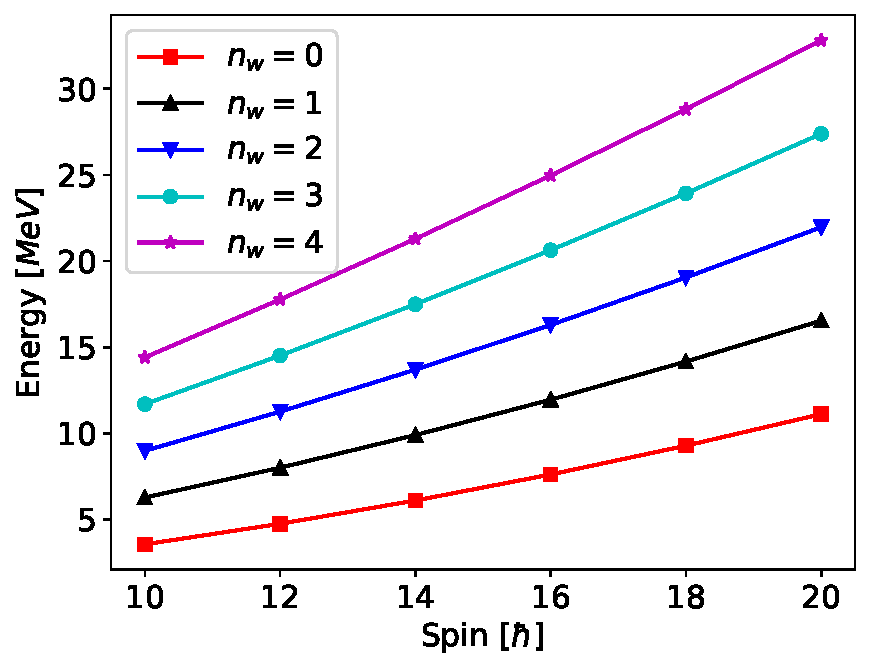
\includegraphics[width=1\linewidth]{figs/simple_wobbling_spectrum.pdf}
  %  \caption{A family of wobbling bands for a triaxial rigid rotor (schematic representation). The calculations were done for $\mathcal{I}_1:\mathcal{I}_2:\mathcal{I}_3=25:5:2$.}
    % \label{simple-wobbling-family}
\end{minipage}%
\begin{minipage}{.4\textwidth}
  \centering
 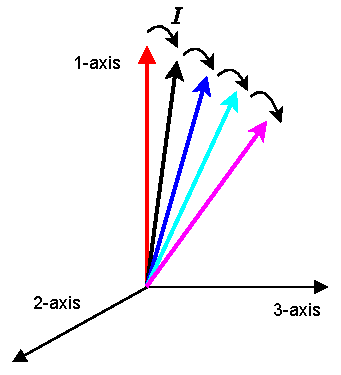
\includegraphics[width=0.85\linewidth]{figs/wobbling_tilting_axis.pdf}
   % \caption{Tilting of the angular momentum away from the rotational axis, with increase in the wobbling phonon excitation.}
    % \label{wobbling-tilt}
\end{minipage}
\caption{Family of wobbling bands for a simple triaxial rotor (left-side). Tilting of the angular momentum vector away from the rotational axis with an increase in spin (right-side). This schematic representation was done for an arbitrary set of MOIs $\mathcal{I}_1:\mathcal{I}_2:\mathcal{I}_3=25:5:2$.}
\label{simple-wobbling-family}
\end{figure}

Just for an illustrative purpose, Figure \ref{simple-wobbling-family} shows a theoretical spectrum for the wobbling bands within a triaxial rigid rotor. The family of wobbling bands is obtained from a set of three moments of inertia (along the three principal axes), a given angular momentum, and increasing wobbling phonon numbers ($n_w=0,1,\dots$). Moreover, in Figure \ref{simple-wobbling-family}, the tilting of the angular momentum away from the rotational axis is sketched, where the tilt increases with the increase in the wobbling excitation. In a given sequence of wobbling bands, both the intra-band $\Delta I=2$ as well as inter-band $\Delta I=1$ transitions have a strong $E2$ collective character.

It is important to mention that the wobbling spectrum described by Eq. \ref{wobbling_eq} and graphically represented in Figure \ref{simple-wobbling-family} was firstly predicted for an even-even triaxial nucleus \cite{bohr1998nuclear}. This predicted wobbling mode has not been experimentally confirmed yet. However, the first experimental evidence for wobbling excitations in nuclei was for an even-odd nucleus, namely $^{163}$Lu, where a single one-phonon wobbling band was measured initially \cite{odegaard2001evidence}, followed by two additional wobbling bands discovered one year later \cite{jensen2002evidence,jensen2002wobbling}.

\subsection{Experimental findings} \label{section2:expdata}

After the first discovery of wobbling bands in $^{163}$Lu ($Z=71$), an entire series of even-odd isotopes with $A\approx160$ were experimentally confirmed as \emph{wobblers}: $^{161}$Lu, $^{165}$Lu, $^{167}$Lu, and $^{167}$Ta. In these nuclei, the wobbling mode appears due to the coupling of a valence nucleon (the so-called $\pi(i_{13/2})$ intruder) to a triaxial core, driving the entire nuclear system up to large deformation ($\epsilon\approx0.4$) \cite{schnack1995superdeformed}.

With time, several nuclei in which WM occurs were also found in regions of smaller $A$. Indeed, two isotopes with $A\approx130$: $^{133}$La \cite{biswas2019longitudinal} and $^{135}$Pr \cite{matta2017transverse,sensharma2019two} were identified as having wobbling bands which emerge from the coupling of a triaxial even-even core with the $\pi(h_{11/2})$ nucleon for $^{135}$Pr, and an additional pair of positive parity quasi-protons for $^{133}$La. In the case of $^{133}$La, the system is characterized as a longitudinal wobbler (it is in fact the first nucleus in which the longitudinal wobbling regime has been experimentally identified), while $^{135}$Pr has a transverse wobbling regime. In both cases, the resulting coupling has a deformation $\epsilon=0.16$ \cite{matta2017transverse,biswas2019longitudinal}, which is smaller than the deformation in the heavier nuclei from the $A\approx160$ region. A third nucleus that also lies in this mass region was confirmed very recently by Chakraborty et. al. in \cite{chakraborty2020multiphonon}, namely the odd-$A$ $^{127}$Xe, where a total of four wobbling bands have been reported by the team (two yrast bands, and two excited phonon bands with $n_w=1$ and $n_w=2$). It is also suggested that $^{131}$Ba could exhibit transverse wobbling \cite{petrache_2018} due to the alignment of a quasiparticle with hole-like character (the $h_{11/2}$ neutron), but in order to support this interpretation, the connecting transitions must show predominant $E2$ character.

Some additional progress was made in the $A\approx100$ mass region, with experimental evidence for $^{105}$Pd with two such bands that are built on a $\nu(h_{11/2})$ configuration, the first one so far in which a valence neutron couples to the triaxial core \cite{timar2019experimental}. The resulting configuration drives the nuclear system up to deformation $\epsilon\approx0.26$ and a transverse wobbling behavior.

The heaviest nuclei known so far in which WM has been experimentally observed are the isotopes $Z=79$ with $A=183$ \cite{nandi2020first} and $A=187$ \cite{sensharma2020longitudinal}, respectively. However, for the case of $^{187}$Au, there is an ongoing investigation \cite{guo2020risk} whether the two wobbling bands ($n_w=0$ and $n_w=1$) are bands with wobbling character, or if they are of magnetic nature (which would exclude the wobbling phonon interpretation). The nucleus $^{183}$Au has probably the most interesting wobbling behavior, due to the appearance of both increasing and decreasing parts of the wobbling energy as a function of angular momentum, for states belonging to the same band (see Figure 5 from \cite{nandi2020first}). The experimental evidence for this nucleus shows that the positive parity band behave as a TW (despite the increasing behavior) due to the geometry of the coupling of the odd quasiparticle. This has important implications which will be discussed later on. For now, it is important to remember that there are cases where some transverse wobblers could be increasing functions of angular momentum, in the low-spin regions.

Regarding the wobbling motion for the even-even nuclei (behavior that was described in Figure \ref{simple-wobbling-family}), the experimental results are fragmentary, with scarce or unclear evidence on this collective behavior. However, some embryos of even-even wobblers have been reported in the recent years. For example, the $^{112}$Ru ($Z=44$) nucleus has three wobbling bands \cite{hamilton2010super}, two of them being the excited one- and two-wobbling phonon bands. Another nucleus is $^{114}$Pd \cite{luo2013triaxial}, with two excited bands of wobbling character, similar to $^{112}$Ru. Indeed, for $^{112}$Ru and $^{114}$Pd the ground band together with the odd and even spin members of the $\gamma$-bands were interpreted as zero-(yrast), one-, and two-phonon wobbling bands. Unfortunately, since there are no data concerning the electromagnetic transitions, its wobbling character is still unclear. The even-even nucleus $^{130}$Ba ($Z=56$) \cite{petrache2019diversity,wang2020two,chen2019transverse} was confirmed very recently to exhibit wobbling behavior based on a two quasiparticle configuration with pair of bands with even and odd spins as zero- and one-phonon wobbling bands, respectively. What is worth noting for this case is the fact that these two bands are built on a configuration in which two aligned protons that emerge from the bottom of $h_{11/2}$ shell couple with the triaxial core. One remarks the change in nature of the wobbling motion from a purely collective form, but in the presence of two aligned quasiparticles \cite{wang2020two}, with a transverse wobbling character. 

Concerning the interpretation of the energy spectrum for the wobbling motion which occurs in the nuclei that were mentioned above, it is mandatory to discuss some aspects related to its behavior with the increase in total angular momentum (nuclear spin). Thus, the concepts of \emph{longitudinal wobblers} (LW) and \emph{transverse wobblers} (TW) emerged from an extensive study done by Frauendorf et. al. \cite{frauendorf2014transverse} in which the team studied the possible coupling schemes that a valence nucleon can create with the triaxial core, giving rise to two possible scenarios. Based on microscopic calculations using the Quasi-Particle Triaxial Rotor (QTR) model, they showed that if the odd valence nucleon aligns its angular momentum vector $\vec{j}$ with the axis of largest MOI, the nuclear system is of longitudinal wobbling character. On the other hand, if the odd nucleon aligns its a.m. vector $\vec{j}$ with an axis perpendicular to the one with the largest MOI, then the nuclear system has a transverse wobbling character. Consequently, for LW the wobbling energy $E_\text{wob}$ (see Eq. \ref{wobbling-energy-relative}) has an \emph{increasing} behavior with an increase in the angular momentum, while for TW the energy $E_\text{wob}$ \emph{decreases} with increasing angular momentum.

From the nuclei that were mentioned above, most of them are of TW type, with only $^{127}$Xe \cite{chakraborty2020multiphonon}, $^{133}$La \cite{biswas2019longitudinal}, and $^{187}$Au \cite{sensharma2020longitudinal} having an LW character. The energy that characterizes the type of wobbling in a nuclear system is the energy of the first excited band (the one-phonon $n_w=1$ wobbling band) relative to the yrast ground band (zero-phonon $n_w=0$ wobbling band):
\begin{align}
    E_\text{wob}(I)=E_{1}(I)-\left(\frac{E_0(I+1)+E_0(I-1)}{2}\right)\ ,
    \label{wobbling-energy-relative}
\end{align}
with 0 and 1 representing the wobbling phonon number $n_w$.

The odd nucleons that couple with the rigid triaxial core will influence the appearance of a particular wobbling regime (LW or TW). In all the wobblers, there is a proton from a certain orbital that is coupling with the core, except for the case of $^{105}$Pd, where the valence nucleon is a neutron. The nature of the odd quasiparticle (i.e., particle or hole) and its "position" in the deformed $j$-shell (i.e., bottom or top) will determine whether its angular momentum $\vec{j}$ will align with the \emph{short} ($s$) or \emph{long} ($l$) axes of the triaxial rotor, respectively (with the notations short $s$, long $l$, and medium $m$ for the axes of a triaxial ellipsoid). The reasoning behind this has to do with the minimization of the overall energy of the system: in the first case, a maximal overlap of its density distribution with the triaxial core will determine a minimal energy, while in the second case, a minimal overlap of the density distribution of the particle with the core will result in a minimal energy. Moreover, if the quasiparticle emerges from the middle of the $j$-shell, then it tends to align its angular momentum vector $\vec{j}$ with the \emph{medium} ($m$) axis of the triaxial core. Figure \ref{quasiparticle-alignment} aims at depicting the type of alignment of a quasiparticle with the triaxial core.

\begin{figure}
    \centering
    % 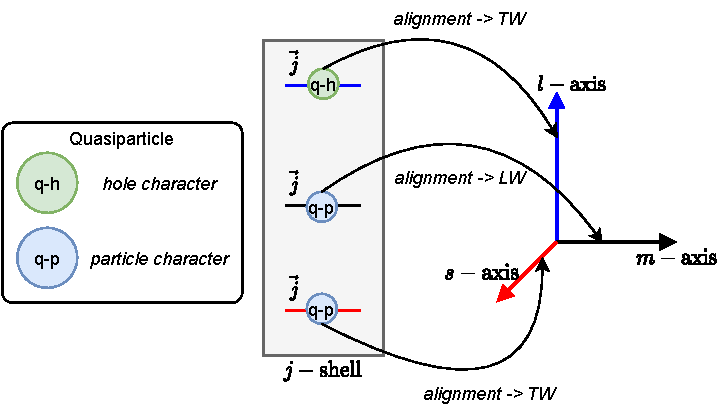
\includegraphics[width=0.85\textwidth]{figs/wobbling_Regimes.pdf}
    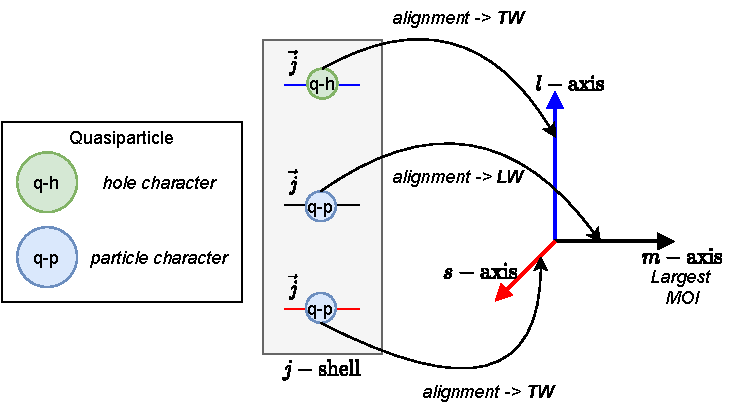
\includegraphics[scale=0.95]{figs/wobbling_Regimes_updated.pdf}
    \caption{The wobbling regimes, Longitudinal Wobbling (LW) or Transverse Wobbling (TW), based on the type of alignment that an odd quasiparticle makes with the principal axes of a triaxial core. Each case depicts a coupling with an odd quasiparticle which emerges from the bottom/middle/top of a $j$-shell \cite{frauendorf2014transverse}.}
    \label{quasiparticle-alignment}
\end{figure}

As previously mentioned, for a given angular momentum, uniform rotation around the axis with the largest MOI corresponds to minimum energy. For a triaxial rotor emerging from a Liquid Drop, this is equivalent to rotation around the $m$ axis. Therefore, Frauendorf \cite{frauendorf2014transverse} classified the LW as the situation when the odd nucleon will align its angular momentum along the $m$-axis, while TW being the situation where $j$ is aligned perpendicular to the $m$-axis (with $s$- or $l$-axis alignment depending on the $j$-shell orbital from which the odd nucleon arises). It is worthwhile to mention the fact that the analysis done in Ref. \cite{frauendorf2014transverse} was performed within a so-called \emph{Frozen Alignment} approximation, where the angular momentum of the odd particle $\vec{j}$ is rigidly aligned with one of the three principal axes of the triaxial ellipsoid (that is $s$-, $l$- or $m$-axis).

For a better understanding of the wobbling regimes in terms of angular momentum alignment, Figure \ref{wobbling-coupling-scheme} depicts three particular cases, namely a simple wobbler - inset A.0 (the case firstly developed by Bohr and Mottelson \cite{bohr1998nuclear}), a longitudinal wobbler - inset A.1, and a transverse wobbler - inset A.2.

\begin{figure}
    \centering
    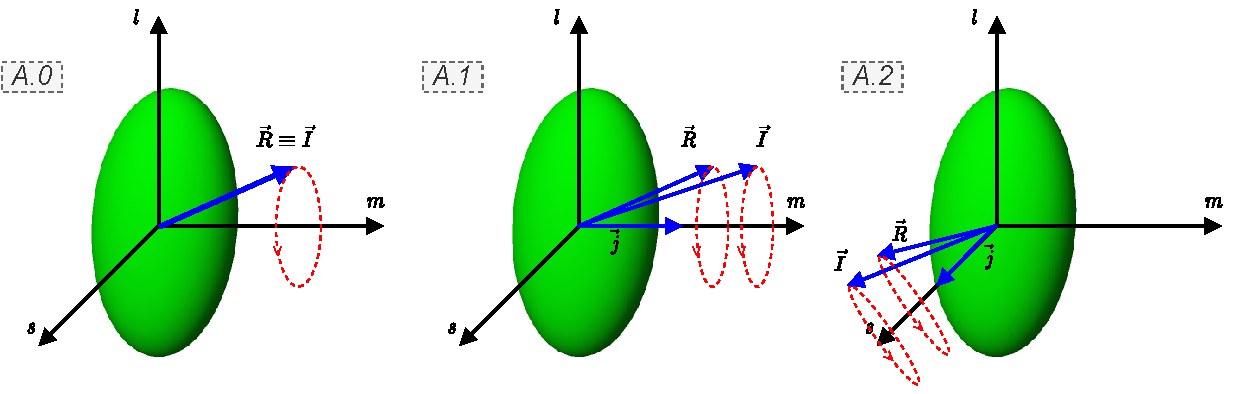
\includegraphics[width=0.9\textwidth]{figs/wobbling_Regimes_COUPLING_SCHEME.pdf}
    \caption{A.0: The geometry for the angular momentum of a simple wobbler. A.1: coupling geometry for a longitudinal wobbler (LW). A.2: coupling geometry for a transverse wobbler (TW). The short-$s$, long-$l$, and medium-$m$ axes are defined in the body-fixed frame. The vectors $\vec{R}$, $\vec{j}$, and $\vec{I}$ represent the set of angular momenta of the core, odd particle, and the total nuclear system, respectively.}
    \label{wobbling-coupling-scheme}
\end{figure}

%\begin{table}[h!t]%
%\caption{This table is taken from RJP volume \textbf{50}(1-2) from page 43 (2005). It gives the ``
%\textit{number of bound states dependence on the radius of space curvature for $\alpha = 0.005$, $U_0 = 1$}''.}
%\centering
%\begin{tabular}{|c|c|}
%\hline
%Value $\rho$ & Value $\varepsilon$ \cr
%\hline
%$\rho = 50$ & -- \cr
%$\rho = 100$ & -- \cr
%$\rho = 250$ & $\varepsilon_1 = 0.0289$ \cr
%$\rho = 400$ & $\varepsilon_1 = 0.3772$ \cr
%$\rho = 1000$ & $\varepsilon_1 = 0.4142$, $\varepsilon_2 = 0.8495$ \cr
%\hline
%\end{tabular}
%\label{table1}
%\end{table}


\begin{acknowledgement}
This work was supported by UEFISCU, through the project \textbf{PCE-16/2021}.
\end{acknowledgement}


\begin{thebibliography}{99}
\bibitem{knuth}D. E. Knuth, D. R. Bibby, ``\textit{The \TeX book}'', 20th edn. (AMS \& Addison-Wesley Publ. Co., 1991).
\bibitem{dknuthhp} D. E. Knuth homepage: \href{http://www-cs-faculty.stanford.edu/~knuth/}{\small\ttfamily www-cs-faculty.stanford.edu/\~{}knuth}.

\end{thebibliography}


\end{document}